\documentclass[rgb]{beamer}

\usepackage[english]{babel}
\usepackage[utf8]{inputenc}
\usepackage{xcolor}
\usepackage{listings}
\usepackage{adjustbox}
\usepackage{amsmath}
\usepackage{multirow}
\usepackage[linewidth=1pt]{mdframed}

% Graphics
\usepackage{graphicx}

\usepackage{tikz}
\usetikzlibrary{calc,shapes.multipart,chains,arrows}

% Font
\usepackage{paratype}
\setbeamerfont{frametitle}{family=\bf}

% Beamer theme settings
\usecolortheme{seagull}
\setbeamertemplate{itemize item}{\raisebox{0.8mm}{\rule{1.8mm}{1.2mm}}}
\usenavigationsymbolstemplate{} % no navigation buttons

\usepackage{listings}

% Define Language
\lstdefinelanguage{fsharp}
{
  % list of keywords
  morekeywords={
    and,
    do,
    else,
    exception,
    for,
    fun,
    function,
    if,
    in,
    let,
    match,
    module,
    mutable,
    open,
    of,
    rec,
    then,
    try,
    type,
    unsafe,
    use,
    val,
    when,
    while,
    with,
  },
  sensitive=true, % keywords are not case-sensitive
  morecomment=[l]{//}, % l is for line comment
%  otherkeywords={>,<,=,<=,>=,!,*,/,-,+,|,&,||,&&,==,=>},
  morestring=[b]" % defines that strings are enclosed in double quotes
}

% Define Colors
\usepackage{color}
\definecolor{eclipseBlue}{RGB}{42,0.0,255}
\definecolor{eclipseGreen}{RGB}{63,127,95}
\definecolor{eclipsePurple}{RGB}{127,0,85}

\newcommand{\fop}[1]{\mbox{\ttfamily\color{eclipseBlue}#1}}
\newcommand{\fw}[1]{\mbox{\ttfamily\bfseries\color{eclipsePurple}#1}}

% Set Language
\lstset{
  language={fsharp},
  basicstyle=\ttfamily, % Global Code Style
  captionpos=b, % Position of the Caption (t for top, b for bottom)
  extendedchars=true, % Allows 256 instead of 128 ASCII characters
  tabsize=2, % number of spaces indented when discovering a tab
  columns=fixed, % make all characters equal width
  keepspaces=true, % does not ignore spaces to fit width, convert tabs to spaces
  showstringspaces=false, % lets spaces in strings appear as real spaces
  breaklines=true, % wrap lines if they don't fit
  frame=trbl, % draw a frame at the top, right, left and bottom of the listing
  frameround=tttt, % make the frame round at all four corners
  framesep=4pt, % quarter circle size of the round corners
  numbers=left, % show line numbers at the left
  numberstyle=\small\ttfamily, % style of the line numbers
  commentstyle=\slshape\bfseries\color{eclipseGreen}, % style of comments
  keywordstyle=\bfseries\color{eclipsePurple}, % style of keywords
  stringstyle=\color{eclipseBlue}, % style of strings
  emph=[1] {
    false,
    true,
    Set,
    Map,
    List,
    ImgUtil,
    Pegs,
    String,
    Array,
    Array2D
  },
  emphstyle=[1]{\color{eclipseBlue}},
  moredelim=**[is][\color{red}]{@@}{@@}
}

\newcommand{\theyear}{2020}
\newcommand{\sem}[1]{[\![#1]\!]}
\newcommand{\seme}[1]{\sem{#1}\varepsilon}
\newcommand{\semzero}[1]{\sem{#1}_0}

\newcommand{\emptymap}{\{\}}
\newcommand{\fracc}[2]{\begin{eqnarray} \frac{\begin{array}{c} #1
    \end{array}}{\begin{array}{c} #2 \end{array}} \end{eqnarray}}
\newcommand{\sembox}[1]{\hfill \normalfont \mbox{\fbox{\(#1\)}}}
\newcommand{\sempart}[2]{\subsubsection*{\rm\em #1 \sembox{#2}}}
\newcommand{\axiom}[1]{\begin{eqnarray} \begin{array}{c} #1 \end{array} \end{eqnarray}}
\newcommand{\fraccn}[2]{\refstepcounter{equation}\mbox{$\frac{\begin{array}{c} #1 \end{array}}{\begin{array}{c} #2 \end{array}}$}~(\arabic{equation})}
\newcommand{\fraccc}[2]{\mbox{$\frac{\begin{array}{c} #1 \end{array}}{\begin{array}{c} #2 \end{array}}$}}
\newcommand{\onepart}[1]{\noindent\hfill#1\hfill~\vspace{2mm}}
\newcommand{\twopart}[2]{\noindent\hfill#1\hfill#2\hfill~\vspace{2mm}}
\newcommand{\threepart}[3]{\noindent\hfill#1\hfill#2\hfill#3\hfill~\vspace{2mm}}
%\newcommand{\axiomm}[1]{\refstepcounter{equation}\mbox{$\begin{array}{c} #1 \end{array}$}~(\arabic{equation})}
\newcommand{\axiomm}[1]{$\begin{array}{c} #1 \end{array}$}
%\newcommand{\ar}[1]{\stackrel{#1}{\longrightarrow}}
\newcommand{\vd}{\vdash}
\newcommand{\Ran}{{\rm Ran}}
\newcommand{\Dom}{{\rm Dom}}
\newcommand{\kw}[1]{\texttt{#1}}
\newcommand{\id}[1]{\mbox{\it{#1}}}
\newcommand{\rarr}{\rightarrow}
\newcommand{\eval}{\rarr}
\newcommand{\evals}{\leadsto}
\newcommand{\larr}{\leftarrow}

\newcommand{\head}[1]{\vspace{3mm} \textbf{\normalsize #1}}
\newcommand{\headsp}[1]{\head{#1}\vspace{1ex}}
\newcommand{\size}{\ensuremath{\mathrm{size}}}
\renewcommand{\log}{\ensuremath{\mathrm{log}}}

\newcommand{\setallthemecolors}[1]{%
\setbeamercolor*{palette primary}{use=structure,fg=white,bg=#1}%
\setbeamercolor*{palette secondary}{use=structure,fg=white,bg=#1}%
\setbeamercolor*{palette tertiary}{use=structure,fg=white,bg=#1}}

\definecolor{black}{RGB}{0,0,0}
\definecolor{maroon}{RGB}{128,0,0}
\definecolor{olive}{RGB}{128,128,0}
\definecolor{green}{RGB}{0,128,0}
\definecolor{purple}{RGB}{128,0,128}
\definecolor{teal}{RGB}{0,128,128}
\definecolor{darkteal}{RGB}{0,92,92}
\definecolor{navy}{RGB}{0,0,128}
\definecolor{gray}{RGB}{128,128,128}
\definecolor{darkgray}{RGB}{60,60,60}
\definecolor{darkred}{RGB}{139,0,0}

%palette

% #173F5F (dark blue)
\definecolor{darkblue}{RGB}{23,63,95}
% #20639B (blue)
\definecolor{blue}{RGB}{32,99,155}
% #3CAEA3 (green)
\definecolor{magenta}{RGB}{60,174,163}
% #F6D55C (yellow)
\definecolor{yellow}{RGB}{246,213,92}
% #ED553B (red)
\definecolor{red}{RGB}{237,85,59}


\usecolortheme{whale}
\useoutertheme{infolines}
\useinnertheme{rectangles}

\newcommand{\popsettitle}[2]{%
\setallthemecolors{#1}%
\newcommand{\popemne}{#2}%
\title{Programmering og Problemløsning}%
\subtitle{#2}%
\author{Martin Elsman}%
\date{}%
\institute[DIKU]{Datalogisk Institut, Københavns Universitet (DIKU)}}

\newcommand{\popmaketitleframe}{%
  \frame{\titlepage%
   \vspace{-15mm}%
   \par\noindent\rule{\textwidth}{0.4pt}%

   \vspace{4mm}%
   \tableofcontents%
   \vspace{-4mm}%
   \par\noindent\rule{\textwidth}{0.4pt}%
  }%
  \section*{\popemne}%
}


\popsettitle{purple}{Typer og Mønstergenkendelse (Del 4)}  % see ../util.tex for colors

\begin{document}

\popmaketitleframe

%%%%%%%%%%%%%%%%%%%%%%%%%%%%%%%%%%%%%%%%%%%%%%%%
%\subsection{Introduktion}
%%%%%%%%%%%%%%%%%%%%%%%%%%%%%%%%%%%%%%%%%%%%%%%%

\begin{frame}[fragile]
\begin{footnotesize}

  \head{Opsamling på Rekursion, Stakke og Kører og Abstrakte typer}

  \vspace{1ex}
  Emner for i dag:

  \vspace{1ex}

\begin{minipage}[b]{0.6\textwidth}

  \begin{enumerate}
  \item \textbf{Opsamling på rekursion.}

    Eksempler på oversættelse af to matematiske definitioner til F\# kode.

  \item \textbf{Stakke og køer.}

    To data-strukturer der let kan implementeres med lister og mønstergenkendelse og hvis
    implementation kan holdes abstrakt ved brug af \textbf{abstrakte
      modul typer}.

  \item \textbf{Introduktion til rekursive sum-typer.}

    Vi vil se på en simpel definition af en træ-struktur i F\#.
  \end{enumerate}
\end{minipage} \hspace{-2mm}
\begin{minipage}[b]{0.3\textwidth}

  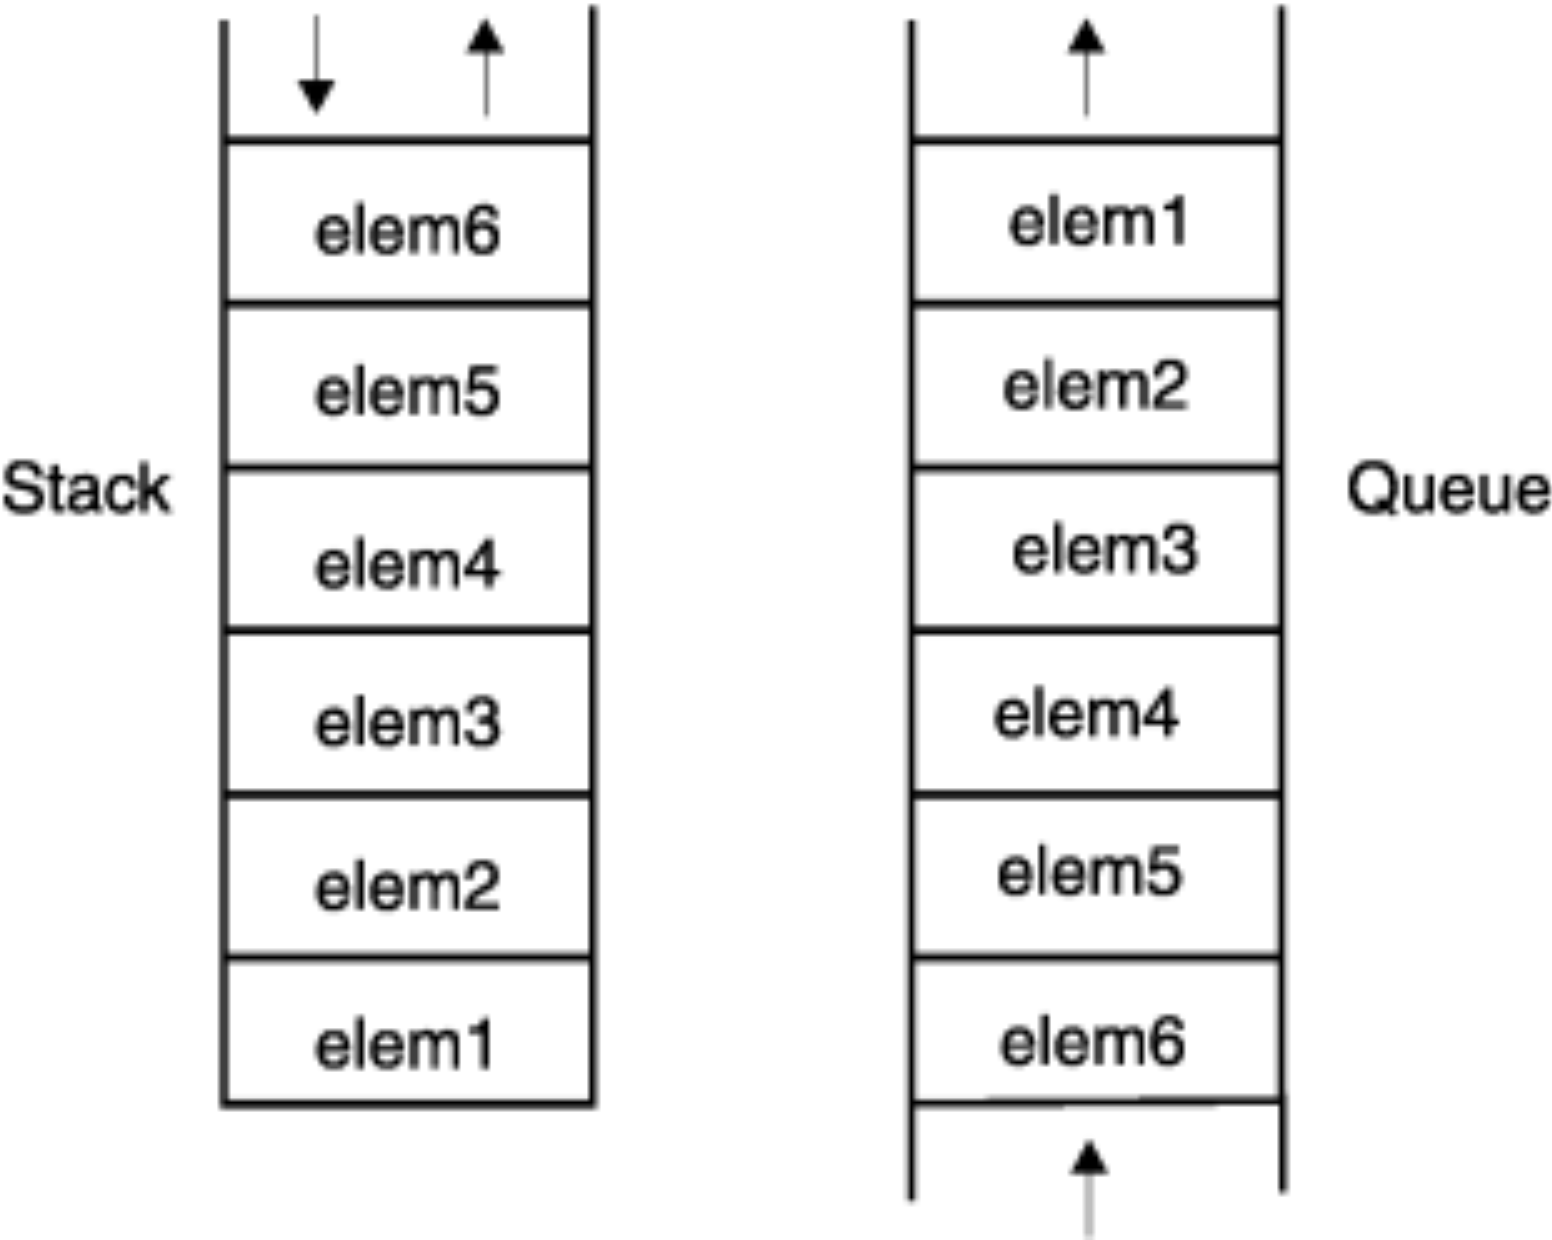
\includegraphics[width=1.4\textwidth]{../images/lifofifo.png}

\end{minipage}

\end{footnotesize}
\end{frame}


\subsection{Opsamling på Rekursion}
\begin{frame}[fragile]
\begin{footnotesize}

  \head{Opsamling på Rekursion}
  \vspace{1ex}

  Vi vil se på hvordan vi kan oversætte to rekursive matematiske formler til F\# kode.

  \vspace{1ex}

  De to eksempler giver sammen mulighed for at beregne ``Maximum Segment
  Sum'' af et heltalsarray, hvor et \emph{segment} er defineret som
  en vilkårlig sammenhængende del af arrayet.

  \vspace{1ex}

  \head{Eksempel:}
\begin{lstlisting}[numbers=none,frame=none,mathescape]
  A = [|-2; 1; -3; $\fbox{\texttt{4; -1; 2; 1}}$; -5; 4|]   // MSS(A) = 6
\end{lstlisting}

  \vspace{1ex}
  \head{Bemærk:}

\begin{itemize}
\item Problemet er kun virkeligt interessant hvis arrayet indeholder negative værdier.
\item Problemet er blandt andet relevant indenfor emner som gen-sekventering, billedgenkendelse og data-mining.
\end{itemize}

\end{footnotesize}
\end{frame}

\begin{frame}[fragile]
\begin{footnotesize}

  \head{Maximum End-Segment Sum}
  \vspace{1ex}

  Vi løser først et nemmere problem:

  \vspace{1ex}

  $\id{MESS}_a(i) = $
  \begin{quote}
    Find det største slut-segment i delarrayet $a[0]..a[i]$.

    dvs: segmentet skal indeholde $a[i]$
  \end{quote}

  \vspace{1ex}

  \head{Eksempel:}
  \vspace{1ex}
\begin{lstlisting}[numbers=none,frame=none,mathescape]
  A = [|-2; 1; -3; $\fbox{\texttt{4; -1}}$; 2; 1; -5; 4|]   // $\id{MESS}_{\mathtt{A}}(4)$ = 3
  //     0  1   2  3   4
\end{lstlisting}
  \vspace{1ex}

  \head{Rekursiv formel:}
  \vspace{1ex}

  \[
  \id{MESS}_a(i) = \left \{ \begin{array}{ll} 0 & \mathrm{if}~i < 0 \\
    \mathrm{max} \left \{ \begin{array}{l} a[i] \\
                                           \id{MESS}_a(i-1)+a[i]
                          \end{array} \right \} & \mathrm{otherwise}. \end{array} \right .
  \]


\end{footnotesize}
\end{frame}

\begin{frame}[fragile]
\begin{footnotesize}

  \head{Maximum End-Segment Sum --- forsat}
  \vspace{1ex}

  \[
  \id{MESS}_a(i) = \left \{ \begin{array}{ll} 0 & \mathrm{if}~i < 0 \\
    \mathrm{max} \left \{ \begin{array}{l} a[i] \\
                                           \id{MESS}_a(i-1)+a[i]
                          \end{array} \right \} & \mathrm{otherwise}. \end{array} \right .
  \]

  \vspace{1ex}

  \head{F\# kode:}
  \vspace{1ex}

\begin{lstlisting}[numbers=none,frame=none,mathescape]
let rec mess (a:int array) i =
  if i < 0 then 0
  else max (a.[i]) (mess a (i-1) + a.[i])

let ex = [|-2; 1; -3; 4; -1; 2; 1; -5; 4|]
do printfn "mess(ex)(4)=%A" (mess ex 4)
\end{lstlisting}

\end{footnotesize}
\end{frame}

\begin{frame}[fragile]
\begin{footnotesize}

  \head{Maximum Segment Sum}
  \vspace{1ex}

  Vi kan nu løse det lidt vanskeligere problem:

  \vspace{1ex}

  $\id{MSS}_a(i) = $
  \begin{quote}
    Find det største segment i en vilkårligt del af delarrayet $a[0]..a[i]$.
  \end{quote}

  \vspace{1ex}

  \head{Eksempel:}
  \vspace{1ex}
\begin{lstlisting}[numbers=none,frame=none,mathescape]
  A = [|-2; 1; -3; $\fbox{\texttt{4}}$; -1; 2; 1; -5; 4|]   // $\id{MSS}_{\mathtt{A}}(4)$ = 4
  //     0  1   2  3   4
\end{lstlisting}
  \vspace{1ex}

  \head{Rekursiv formel:}
  \vspace{1ex}

  \[
  \id{MSS}_a(i) = \left \{ \begin{array}{ll} 0 & \mathrm{if}~i < 0 \\
    \mathrm{max} \left \{ \begin{array}{l} \id{MESS}_a(i) \\
                                           \id{MSS}_a(i-1)
                          \end{array} \right \} & \mathrm{otherwise}. \end{array} \right .
  \]


\end{footnotesize}
\end{frame}

\begin{frame}[fragile]
\begin{footnotesize}

  \head{Maximum Segment Sum --- forsat}
  \vspace{1ex}

  \[
  \id{MSS}_a(i) = \left \{ \begin{array}{ll} 0 & \mathrm{if}~i < 0 \\
    \mathrm{max} \left \{ \begin{array}{l} \id{MESS}_a(i) \\
                                           \id{MSS}_a(i-1)
                          \end{array} \right \} & \mathrm{otherwise}. \end{array} \right .
  \]

  \head{F\# kode:}
  \vspace{1ex}

\begin{lstlisting}[numbers=none,frame=none,mathescape]
let rec mss (a:int array) i =
  if i < 0 then 0
  else max (mess a i)        // max segment at end
           (mss a (i-1))     // max segment somewhere before

let ex = [|-2; 1; -3; $\fbox{\texttt{4; -1; 2; 1}}$; -5; 4|]
do printfn "mss(ex)(|ex|-1)=%A" (mss ex (Array.length ex - 1))
\end{lstlisting}

\end{footnotesize}
\end{frame}

\subsection{Stakke og Køer}
\begin{frame}[fragile]
\begin{footnotesize}

  \head{Stakke}

  \vspace{1ex}

\begin{minipage}[b]{0.80\textwidth}

  En \emph{stak} er en data-struktur med et simpelt interface:

  \vspace{1ex}

\begin{lstlisting}[numbers=none,frame=none,mathescape]
module Stack // content of stack.fsi

type 'a stack                          // LIFO
val empty : unit -> 'a stack
val push  : 'a stack -> 'a -> 'a stack
val pop   : 'a stack -> ('a * 'a stack) option
\end{lstlisting}
  \vspace{1ex}
  \head{Spørgsmål:}
\begin{itemize}
\item Hvordan implementers et stak-modul?
\item Hvordan sikres det at man \textbf{KUN} kan tilgå værdier af type
  \lstinline{'a stack} med operationerne \lstinline{pop} og
  \lstinline{push}?
\end{itemize}

\end{minipage} \hspace{-8mm}
\begin{minipage}[b]{0.16\textwidth}

  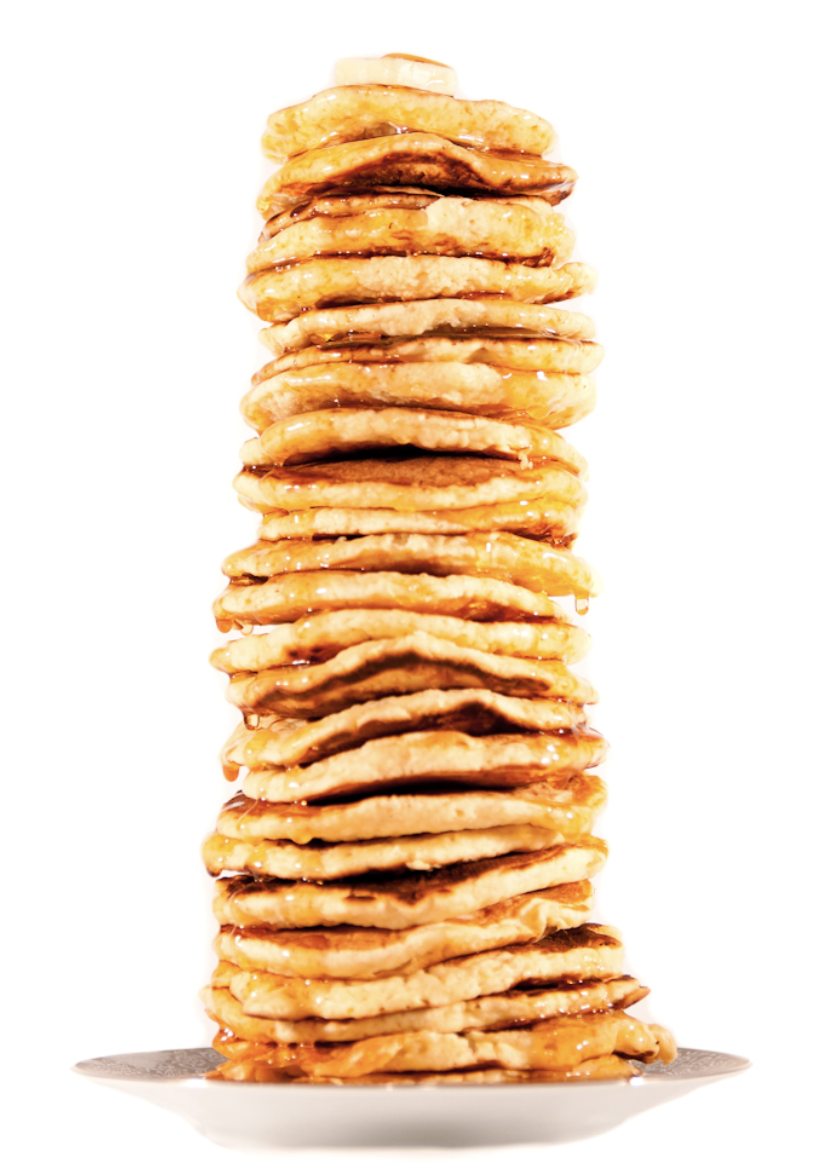
\includegraphics[width=1.8\textwidth]{../images/stack.png}

\end{minipage}

\end{footnotesize}
\end{frame}

\begin{frame}[fragile]
\begin{footnotesize}

  \head{Stak-implementation}

  \vspace{1ex}


\begin{lstlisting}[numbers=none,frame=none,mathescape]
module Stack

type 'a stack = S of 'a list
let empty () = S []
let push (S s: 'a stack) v = S (v::s)
let pop (S s) : ('a * 'a stack) option =
  match s with
    | [] -> None
    | x::xs -> Some (x,S xs)
\end{lstlisting}

  \vspace{1ex}
  \head{Bemærk:}
\begin{itemize}
\item Enkel version ved brug af \lstinline{'a list}.
\item Singleton ``Sum-type'' benyttes til at sikre \textbf{fuld abstraktion} (\lstinline{S} konstruktør) .
\item Modul skal oversættes med både fsi-fil og fs-fil:
\begin{verbatim}
$ fsharpc -a stack.fsi stack.fs
$ fsharpi -r stack.dll
\end{verbatim}
\end{itemize}

\end{footnotesize}
\end{frame}

\begin{frame}[fragile]
\begin{footnotesize}

  \head{Køer}

  \vspace{1ex}

\begin{minipage}[b]{0.80\textwidth}

  En \emph{kø} er en data-struktur med et simpelt interface:

  \vspace{1ex}

\begin{lstlisting}[numbers=none,frame=none,mathescape]
module Queue // content of queue.fsi

type 'a queue                        // FIFO
val empty : unit -> 'a queue
val insert  : 'a queue -> 'a -> 'a queue
val remove  : 'a queue -> ('a * 'a queue) option
\end{lstlisting}
  \vspace{1ex}
  \head{Spørgsmål:}
\begin{itemize}
\item Hvordan implementers et kø-modul?
\item Hvordan sikres det at man \textbf{KUN} kan tilgå værdier af type
  \lstinline{'a queue} med operationerne \lstinline{insert} og
  \lstinline{remove}?
\end{itemize}

\end{minipage} \hspace{-4mm}
\begin{minipage}[b]{0.16\textwidth}

  
\includegraphics[width=1.4\textwidth,height=3cm]{../images/queue.png}

\end{minipage}

\end{footnotesize}
\end{frame}

\begin{frame}[fragile]
\begin{footnotesize}

  \head{Kø-implementation --- NOT GOOD --- file \texttt{queue\_bad.fs}}

  \vspace{1ex}

\begin{lstlisting}[numbers=none,frame=none,mathescape]
module Queue

type 'a queue = Q of 'a list                 // BAD
let empty () = Q []                          // BAD
let insert (Q q: 'a queue) v = Q (v::s)      // BAD
let remove (Q q) : ('a * 'a queue) option =  // BAD
  match List.rev q with                      // BAD
    | [] -> None                             // BAD
    | x::xs -> Some (x,Q (List.rev xs))      // BAD
\end{lstlisting}

  \vspace{1ex}
  \head{Bemærk:}
\begin{itemize}
\item Enkel version ved brug af \lstinline{'a list}.
\item Singleton ``Sum-type'' benyttes til at sikre \textbf{fuld abstraktion} (\lstinline{Q} konstruktør) .
\end{itemize}

  \vspace{1ex}
  \head{Spørgsmål:}
  \begin{itemize}
  \item Hvad er problemet?
\end{itemize}

\end{footnotesize}
\end{frame}

\begin{frame}[fragile]
\begin{footnotesize}

  \head{Kø-test --- file \texttt{qtest.fs}}

  \vspace{1ex}

\begin{lstlisting}[numbers=none,frame=none,mathescape]
  module Q = Queue
  let q = List.fold (fun q v -> Q.insert q v) (Q.empty()) [0..5000]
  let rec loop q = match Q.remove q with
                     | None -> 0
                     | Some (v,q) -> v + loop q
  let a = loop q
  do printfn "sum(queue) = %d" a
\end{lstlisting}

  \vspace{1ex}

\head{Kørsel med \texttt{queue\_bad.fs}}
\begin{verbatim}
cp queue_bad.fs queue.fs
fsharpc --nologo -a queue.fsi queue.fs
fsharpc --nologo -r queue.dll qtest.fs
time mono qtest.exe
sum(queue) = 12502500
        3.60 real         4.12 user         0.14 sys
\end{verbatim}
\end{footnotesize}
\end{frame}

\begin{frame}[fragile]
\begin{footnotesize}

  \head{En bedre kø-implementation --- file \texttt{queue\_good.fs}}

  \vspace{1ex}

\begin{lstlisting}[numbers=none,frame=none,mathescape]
module Queue     // GOOD Queue Implementation

type 'a queue = Q of 'a list * 'a list
let empty () = Q ([],[])
let insert (Q (b,f)) v = Q (v::b,f)
let remove (Q (b,f)) : ('a * 'a queue) option =
  match f with
    | x :: xs -> Some (x,Q(b,xs))
    | [] ->
      match List.rev b with
        | [] -> None
        | x :: xs -> Some (x,Q([],xs))
\end{lstlisting}

  \vspace{1ex}
  \head{Bemærk:}
\begin{itemize}
\item To lister: en til ``indsættelse'' og en til ``fjernelse''.
\item Hvis listen til fjernelse er tom tages hele listen til
  indsættelse og indsættes i listen til fjernelse (efter at den er
  vendt om).
\end{itemize}

\end{footnotesize}
\end{frame}

\begin{frame}[fragile]
\begin{footnotesize}

\head{Kørsel af \texttt{qtest.fs} med \texttt{queue\_good.fs}}
  \vspace{1ex}

\begin{verbatim}
cp queue_good.fs queue.fs
fsharpc --nologo -a queue.fsi queue.fs
fsharpc --nologo -r queue.dll qtest.fs
time mono qtest.exe
sum(queue) = 12502500
        0.06 real         0.04 user         0.00 sys
\end{verbatim}

  \vspace{1ex}
  \head{Bemærk:}
\begin{itemize}
\item Vi har formået at ændre implementationen af kø-modulet uden at programmet \texttt{qtest.fs} kan ``se forskel''.
\item Applikationen virker stadig korrekt (hvilket kunne testes med black-box unit testing).
\item Effekten er blot at programmet \texttt{qtest.fs} nu kører hurtigere!

  (Før 3 sekunder nu 60 millisekunder...)
\end{itemize}

\end{footnotesize}
\end{frame}

\end{document}
